\documentclass[11pt,a4paper]{article}

\usepackage[utf8]{inputenc}
\usepackage[T1]{fontenc}
\usepackage[margin=2.5cm]{geometry}
\usepackage{amsmath,amssymb,amsthm}
\usepackage{enumitem}
\usepackage{tikz}
\usepackage{array}
\usepackage{booktabs}
\usepackage{fancyhdr}
\usepackage{titlesec}
\usepackage{xcolor}
\usepackage[colorlinks=true,linkcolor=black,urlcolor=blue]{hyperref}

\usetikzlibrary{positioning,arrows.meta,calc}

% ---------- Pengaturan tampilan ----------
\pagestyle{fancy}
\fancyhf{}
\fancyhead[L]{\small Matematika Diskrit}
\fancyhead[R]{\small Latihan Soal}
\fancyfoot[C]{\thepage}
\renewcommand{\headrulewidth}{0.4pt}

\titleformat{\section}{\large\bfseries\color{blue!50!black}}{\thesection.}{0.6em}{}
\titlespacing*{\section}{0pt}{16pt}{8pt}

\newcommand{\soal}[2]{%
  \vspace{4pt}\noindent\textbf{Soal #1.}\ \textit{(#2)}\par\nobreak\vspace{2pt}}

\newcommand{\jawab}[1]{\vspace{4pt}\noindent\textbf{Jawaban #1.}\par\nobreak\vspace{2pt}}

\DeclareMathOperator{\lcmop}{lcm}
\DeclareMathOperator{\Deg}{deg}
\newcommand{\Comp}[1]{\overline{#1}}
\newcommand{\Zset}{\mathbb{Z}}
\newcommand{\Nset}{\mathbb{N}}

\setlist[enumerate,2]{label=(\alph*),leftmargin=*}

% ---------- Judul ----------
\title{\vspace{-1.5cm}\textbf{Latihan Soal Matematika Diskrit}\\[4pt]
\large 15 Soal: 5 Mudah, 5 Sedang, 5 Sulit}
\author{}
\date{}

\begin{document}
\maketitle
\vspace{-1.8cm}

\begin{center}
\begin{tabular}{ll}

\end{tabular}
\end{center}

\vspace{6pt}

\section*{BAGIAN A .Tingkat Mudah}
\addcontentsline{toc}{section}{Bagian A}

\soal{1}{Logika dan Penalaran}
Diberikan ekspresi logika
\[
F(p,q,r) \;=\; (p \rightarrow q) \wedge (\neg p \rightarrow r).
\]
\begin{enumerate}[label=(\alph*),leftmargin=*]
  \item Susun tabel kebenaran lengkap untuk $F$ (8 baris).
  \item Tentukan apakah $F$ merupakan tautologi, kontradiksi, atau kontingensi.
  \item Buktikan bahwa $\big[(p \rightarrow q) \wedge \neg q\big] \rightarrow \neg p$ adalah tautologi
        \emph{tanpa} menggunakan tabel kebenaran, yaitu dengan menerapkan hukum-hukum
        ekuivalensi logika.
\end{enumerate}

\soal{2}{Himpunan}
Misalkan semesta pembicaraan $U = \{1,2,3,\dots,12\}$ dan
\[
A = \{x \in U : 2 \mid x\}, \qquad
B = \{x \in U : 3 \mid x\}, \qquad
C = \{x \in U : x \text{ bilangan prima}\}.
\]
\begin{enumerate}[label=(\alph*),leftmargin=*]
  \item Daftarkan anggota $A$, $B$, dan $C$, lalu tentukan
        $A \cap B$, $A \cup C$, dan $(A - B) \cap C$.
  \item Hitung $|\mathcal{P}(A \cap B)|$, yaitu kardinalitas himpunan kuasa dari $A \cap B$.
  \item Verifikasi hukum De Morgan $\Comp{A \cup B} = \Comp{A} \cap \Comp{B}$
        dengan mendaftarkan anggota kedua ruas.
\end{enumerate}

%------------------------------------------------- 3
\soal{3}{Relasi dan Fungsi}
\begin{enumerate}[label=(\alph*),leftmargin=*]
  \item Pada himpunan $A = \{1,2,3,4\}$ didefinisikan relasi
  \[
  R = \{(1,1),(1,2),(2,1),(2,2),(3,3),(3,4),(4,3),(4,4)\}.
  \]
  Periksa sifat refleksif, simetris, antisimetris, dan transitif dari $R$.
  Apakah $R$ merupakan relasi ekivalen? Jika ya, tuliskan semua kelas ekivalensinya.
  \item Diberikan $f : \Zset \rightarrow \Zset$ dengan $f(x) = 2x + 3$.
  Tentukan apakah $f$ injektif dan/atau surjektif. Berikan bukti singkat untuk
  setiap klaim.
\end{enumerate}

%------------------------------------------------- 4
\soal{4}{Teori Bilangan}
\begin{enumerate}[label=(\alph*),leftmargin=*]
  \item Gunakan algoritma Euclid untuk menghitung $\gcd(1071, 462)$.
        Tuliskan setiap langkah pembagiannya.
  \item Dengan memakai hasil (a), tentukan $\lcmop(1071, 462)$.
  \item Tentukan nilai $3^{100} \bmod 7$. Jelaskan strategi yang dipakai
        (jangan menghitung $3^{100}$ secara langsung).
\end{enumerate}

%------------------------------------------------- 5
\soal{5}{Kombinatorika}
\begin{enumerate}[label=(\alph*),leftmargin=*]
  \item Sebuah \emph{password} terdiri atas tepat 6 karakter yang diambil dari
        26 huruf kecil dan 10 digit (karakter boleh berulang).
        Berapa banyak password yang memuat \emph{sekurang-kurangnya satu digit}?
  \item Berapa banyak susunan huruf berbeda yang dapat dibentuk dari
        seluruh huruf pada kata \textbf{MATEMATIKA}?
\end{enumerate}

%=====================================================================
\section*{BAGIAN B --- Tingkat Sedang}

%------------------------------------------------- 6
\soal{6}{Induksi Matematika}
\begin{enumerate}[label=(\alph*),leftmargin=*]
  \item Buktikan dengan induksi matematika bahwa untuk setiap bilangan bulat $n \ge 1$,
  \[
  \sum_{i=1}^{n} i \cdot 2^{i} \;=\; (n-1)\,2^{\,n+1} + 2 .
  \]
  \item Buktikan dengan induksi kuat bahwa setiap bilangan bulat $n \ge 12$ dapat
  dinyatakan sebagai $n = 4a + 5b$ untuk suatu bilangan bulat tak negatif $a$ dan $b$.
  Jelaskan mengapa basis induksinya harus terdiri atas lebih dari satu nilai.
  \item Katakan $F_1,F_2,\dots$ adalah barisan fibonacci. Buktikan dengan induksi bahwa
  \[
  F_{n+m} = F_{n-1}F_m + F_nF_{m+1}
  \]
\end{enumerate}

%------------------------------------------------- 7
\soal{7}{Aljabar Boolean}
Diberikan fungsi Boolean empat peubah
\[
f(A,B,C,D) \;=\; \sum m(0,1,2,5,8,9,10).
\]
\begin{enumerate}[label=(\alph*),leftmargin=*]
  \item Tuliskan bentuk kanonik SOP (\emph{sum of products}) dari $f$ dalam notasi literal.
  \item Sederhanakan $f$ menggunakan peta Karnaugh $4\times4$.
        Gambarkan petanya dan tandai setiap kelompok (\emph{prime implicant})
        yang Anda pakai.
  \item Sebutkan \emph{prime implicant} mana yang bersifat esensial, dan hitung
        berapa banyak gerbang AND/OR yang dibutuhkan pada rangkaian hasil
        penyederhanaan (abaikan gerbang NOT).
\end{enumerate}

%------------------------------------------------- 8
\soal{8}{Barisan, Sumasi, dan Relasi Rekurens}
\begin{enumerate}[label=(\alph*),leftmargin=*]
  \item Selesaikan relasi rekurens homogen linear
  \[
  a_n = 5a_{n-1} - 6a_{n-2}, \qquad a_0 = 1,\; a_1 = 4,
  \]
  dengan metode persamaan karakteristik. Verifikasi hasilnya untuk $n = 2$.
  \item Selesaikan relasi rekurens tak homogen
  \[
  b_n = 2b_{n-1} + 3, \qquad b_0 = 1,
  \]
  dengan mencari solusi homogen dan solusi partikular.
\end{enumerate}

%------------------------------------------------- 9
\soal{9}{Kompleksitas Algoritma}
\begin{enumerate}[label=(\alph*),leftmargin=*]
  \item Tentukan kompleksitas waktu asimtotik (dalam notasi $\Theta$) dari potongan
  algoritma berikut, disertai perhitungan jumlah operasi \texttt{x++}:
  \begin{quote}
  \ttfamily
  for (i = 1; i <= n; i = i * 2)\\
  \hspace*{1.5em}for (j = 1; j <= i; j = j + 1)\\
  \hspace*{3em}x++;
  \end{quote}
  \item Buktikan langsung dari definisi formal notasi $O$ bahwa
  \[
  3n^{3} + 5n^{2}\log n + 7 \;=\; O(n^{3}),
  \]
  yaitu tunjukkan konstanta $c > 0$ dan $n_0$ yang memenuhi definisi.
  \item Selesaikan relasi rekurens $T(n) = 2\,T(n/2) + n\log n$ dengan $T(1) = 1$
  (asumsikan $n = 2^{k}$) menggunakan metode pohon rekursi, dan nyatakan hasilnya
  dalam notasi $\Theta$.
\end{enumerate}

%------------------------------------------------- 10
\soal{10}{Graf}
Diberikan graf sederhana $G = (V,E)$ dengan
\[
V = \{a,b,c,d,e\}, \qquad
E = \{ab,\; ac,\; bc,\; bd,\; cd,\; ce,\; de\}.
\]

\begin{center}
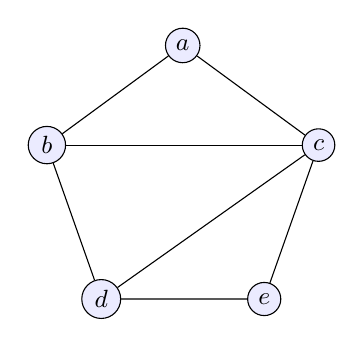
\begin{tikzpicture}[every node/.style={circle,draw,fill=blue!8,inner sep=2.2pt,font=\small},scale=1.15]
  \node (a) at (0,1.6) {$a$};
  \node (b) at (-1.5,0.5) {$b$};
  \node (c) at (1.5,0.5) {$c$};
  \node (d) at (-0.9,-1.2) {$d$};
  \node (e) at (0.9,-1.2) {$e$};
  \draw (a)--(b); \draw (a)--(c); \draw (b)--(c);
  \draw (b)--(d); \draw (c)--(d); \draw (c)--(e); \draw (d)--(e);
\end{tikzpicture}
\end{center}

\begin{enumerate}[label=(\alph*),leftmargin=*]
  \item Tuliskan derajat setiap simpul dan verifikasi \emph{handshaking lemma}.
  \item Tentukan apakah $G$ memiliki sirkuit Euler dan/atau lintasan Euler.
        Jika ada, tuliskan satu contohnya secara eksplisit.
  \item Tentukan apakah $G$ memiliki sirkuit Hamilton. Jika ada, tuliskan satu contohnya.
  \item Apakah $G$ merupakan graf bipartit? Buktikan jawaban Anda.
\end{enumerate}

%=====================================================================
\section*{BAGIAN C --- Tingkat Sulit}

%------------------------------------------------- 11
\soal{11}{Teori Bilangan, Anti LLM}
Mbappe sedang memainkan sebuah permainan yang lumayan membingungkan. Awalnya dia diberikan sebuah bilangan asli $n$. Dalam tiap giliran dia dapat memilih salah satu operasi, yaitu \begin{enumerate}
    \item mengalikan $n$ dengan sembarang bilangan bulat positif $x$,
    \item atau mengubah $n$ menjadi $\sqrt n$ (disini, nilai $n$ sekarang harus merupakan bilangan kuadrat).
\end{enumerate}  
Mbappe ingin mengetahui nilai $n$ terkecil apa yang bisa ia peroleh dan langkah minimum supaya sampai ke nilai tersebut. Selesaikan permasalahan - permasalahan berikut : 
\begin{enumerate}[label=(\alph*),leftmargin=*]
    \item Jika $n = 5184$, tentukan jawabannya!
    \item Jika diberikan faktoriasi prima dari $n = p_1^{a_1}\cdot p_2^{a_2}\cdot\dots\cdot p_k^{a_k}$, dimana $p_i \neq p_j$ untuk setiap $i\neq j$, tentukan jawaban dalam variabel - variabel yang diketahui.
\end{enumerate}


%------------------------------------------------- 12
\soal{12}{Teori Bilangan Lanjut}
\begin{enumerate}[label=(\alph*),leftmargin=*]
  \item Selesaikan sistem kongruensi berikut dengan \emph{Chinese Remainder Theorem}:
  \[
  x \equiv 2 \pmod 3, \qquad x \equiv 3 \pmod 5, \qquad x \equiv 2 \pmod 7.
  \]
  Tuliskan solusi umum dan solusi positif terkecilnya.
  \item Pada skema RSA dipilih $p = 11$, $q = 13$, dan $e = 7$.
  \begin{enumerate}[label=(\roman*)]
    \item Hitung $n$ dan $\varphi(n)$, lalu verifikasi bahwa $e$ merupakan pilihan yang sah.
    \item Tentukan kunci privat $d$ menggunakan algoritma Euclid diperluas.
    \item Enkripsi pesan $M = 9$, yaitu hitung $C = M^{e} \bmod n$ dengan
          teknik \emph{fast modular exponentiation}.
  \end{enumerate}
\end{enumerate}

%------------------------------------------------- 13
\soal{13}{Kombinatorika Lanjut}
\begin{enumerate}[label=(\alph*),leftmargin=*]
  \item Dengan prinsip inklusi--eksklusi, hitung banyaknya bilangan bulat pada
  $\{1,2,\dots,1000\}$ yang \emph{tidak} habis dibagi 2, 3, maupun 5.
  \item Hitung banyaknya fungsi surjektif dari himpunan berukuran 6 ke himpunan
  berukuran 3. Turunkan rumus umumnya terlebih dahulu dengan inklusi--eksklusi.
  \item Buktikan dengan prinsip \emph{pigeonhole}: jika dipilih 10 bilangan bulat
  berbeda dari $\{1,2,\dots,100\}$, maka selalu terdapat dua himpunan bagian tak
  kosong yang saling lepas dan memiliki jumlah anggota yang sama.
\end{enumerate}

%------------------------------------------------- 14
\soal{14}{Pohon}
\begin{enumerate}[label=(\alph*),leftmargin=*]
  \item Sebuah pohon biner memiliki hasil penelusuran
  \[
  \text{preorder}: A\;B\;D\;E\;C\;F\;G, \qquad
  \text{inorder}: D\;B\;E\;A\;F\;C\;G .
  \]
  Rekonstruksi pohon tersebut dan tentukan hasil penelusuran \emph{postorder}-nya.
  \item Buktikan bahwa sebuah pohon $m$-ari penuh dengan $i$ simpul internal
  memiliki $n = m\,i + 1$ simpul seluruhnya dan $\ell = (m-1)\,i + 1$ daun.
  \item Diberikan graf berbobot $H$ berikut. Tentukan pohon merentang minimum (MST)
  beserta bobot totalnya menggunakan algoritma Kruskal. Tuliskan urutan sisi yang
  diperiksa, dan tandai sisi mana yang ditolak karena membentuk sirkuit.

  \begin{center}
  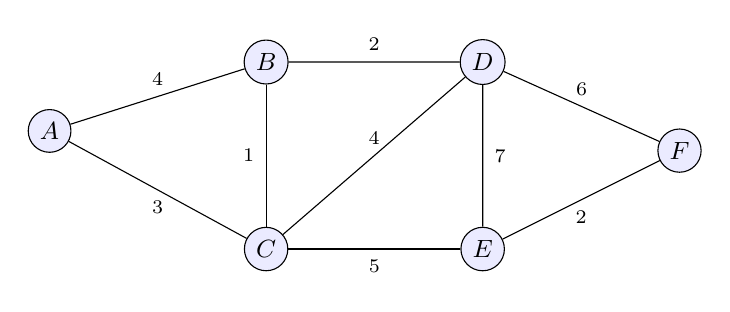
\begin{tikzpicture}[every node/.style={circle,draw,fill=blue!8,inner sep=2.2pt,font=\small},
                      every label/.style={draw=none,fill=none,font=\scriptsize},scale=1.25]
    \node (A) at (-2.2,1.2) {$A$};
    \node (B) at (0,1.9) {$B$};
    \node (C) at (0,0) {$C$};
    \node (D) at (2.2,1.9) {$D$};
    \node (E) at (2.2,0) {$E$};
    \node (F) at (4.2,1.0) {$F$};
    \draw (A)--(B) node[midway,above,draw=none,fill=none,font=\scriptsize]{4};
    \draw (A)--(C) node[midway,below,draw=none,fill=none,font=\scriptsize]{3};
    \draw (B)--(C) node[midway,left,draw=none,fill=none,font=\scriptsize]{1};
    \draw (B)--(D) node[midway,above,draw=none,fill=none,font=\scriptsize]{2};
    \draw (C)--(D) node[midway,above,draw=none,fill=none,font=\scriptsize]{4};
    \draw (C)--(E) node[midway,below,draw=none,fill=none,font=\scriptsize]{5};
    \draw (D)--(E) node[midway,right,draw=none,fill=none,font=\scriptsize]{7};
    \draw (D)--(F) node[midway,above,draw=none,fill=none,font=\scriptsize]{6};
    \draw (E)--(F) node[midway,below,draw=none,fill=none,font=\scriptsize]{2};
  \end{tikzpicture}
  \end{center}
\end{enumerate}

%------------------------------------------------- 15
\soal{15}{Pewarnaan Graf}
\begin{enumerate}[label=(\alph*),leftmargin=*]
  \item Buktikan dengan induksi pada banyaknya simpul bahwa untuk setiap graf
  sederhana $G$ berlaku $\chi(G) \le \Delta(G) + 1$, dengan $\Delta(G)$ derajat
  maksimum $G$.
  \item Tentukan bilangan kromatik dari $K_{3,4}$, $C_{7}$, dan graf roda $W_{5}$
  (yaitu $C_5$ ditambah satu simpul pusat yang terhubung ke semua simpul siklus).
  Jelaskan alasannya masing-masing.
  \item Tujuh mata kuliah $M_1, \dots, M_7$ akan dijadwalkan ujiannya. Dua mata
  kuliah tidak boleh berada pada slot yang sama jika ada mahasiswa yang mengambil
  keduanya. Daftar konflik:
  \[
  \{M_1M_2,\; M_1M_3,\; M_1M_4,\; M_2M_3,\; M_2M_5,\; M_3M_4,\;
    M_3M_6,\; M_4M_5,\; M_4M_6,\; M_5M_6,\; M_5M_7,\; M_6M_7\}.
  \]
  Modelkan sebagai masalah pewarnaan graf, tentukan jumlah slot ujian minimum,
  dan berikan satu penjadwalan yang valid. Buktikan bahwa jumlah tersebut memang
  minimum.

\end{enumerate}

\clearpage
%=====================================================================
\section*{KUNCI JAWABAN DAN PEMBAHASAN}
%=====================================================================

\jawab{1}
\textbf{(a)} Tabel kebenaran $F = (p \rightarrow q) \wedge (\neg p \rightarrow r)$:

\begin{center}
\begin{tabular}{cccccc}
\toprule
$p$ & $q$ & $r$ & $p \rightarrow q$ & $\neg p \rightarrow r$ & $F$\\
\midrule
T & T & T & T & T & \textbf{T}\\
T & T & F & T & T & \textbf{T}\\
T & F & T & F & T & F\\
T & F & F & F & T & F\\
F & T & T & T & T & \textbf{T}\\
F & T & F & T & F & F\\
F & F & T & T & T & \textbf{T}\\
F & F & F & T & F & F\\
\bottomrule
\end{tabular}
\end{center}

\textbf{(b)} $F$ bernilai T pada 4 baris dan F pada 4 baris, jadi $F$ adalah
\textbf{kontingensi}.

\textbf{(c)} Modus tollens:
\begin{align*}
\big[(p \rightarrow q) \wedge \neg q\big] \rightarrow \neg p
&\equiv \neg\big[(\neg p \vee q) \wedge \neg q\big] \vee \neg p && \text{(implikasi)}\\
&\equiv \big[\neg(\neg p \vee q) \vee q\big] \vee \neg p && \text{(De Morgan)}\\
&\equiv \big[(p \wedge \neg q) \vee q\big] \vee \neg p && \text{(De Morgan)}\\
&\equiv \big[(p \vee q) \wedge (\neg q \vee q)\big] \vee \neg p && \text{(distributif)}\\
&\equiv (p \vee q) \vee \neg p && \text{(negasi: } \neg q \vee q \equiv \mathrm{T})\\
&\equiv (p \vee \neg p) \vee q \;\equiv\; \mathrm{T} \vee q \;\equiv\; \mathrm{T}.
\end{align*}
Terbukti tautologi. $\blacksquare$

\jawab{2}
\textbf{(a)} $A = \{2,4,6,8,10,12\}$, $B = \{3,6,9,12\}$, $C = \{2,3,5,7,11\}$.
\begin{itemize}[leftmargin=*,nosep]
  \item $A \cap B = \{6,12\}$
  \item $A \cup C = \{2,3,4,5,6,7,8,10,11,12\}$
  \item $A - B = \{2,4,8,10\}$ sehingga $(A-B) \cap C = \{2\}$
\end{itemize}

\textbf{(b)} $|A \cap B| = 2$, maka $|\mathcal{P}(A \cap B)| = 2^{2} = \mathbf{4}$.

\textbf{(c)} $A \cup B = \{2,3,4,6,8,9,10,12\}$, maka $\Comp{A \cup B} = \{1,5,7,11\}$.
Di sisi lain $\Comp{A} = \{1,3,5,7,9,11\}$ dan $\Comp{B} = \{1,2,4,5,7,8,10,11\}$,
sehingga $\Comp{A} \cap \Comp{B} = \{1,5,7,11\}$. Kedua ruas sama. $\blacksquare$

\jawab{3}
\textbf{(a)}
\begin{itemize}[leftmargin=*,nosep]
  \item \emph{Refleksif}: $(1,1),(2,2),(3,3),(4,4) \in R$ $\Rightarrow$ ya.
  \item \emph{Simetris}: $(1,2)$ dan $(2,1)$ ada; $(3,4)$ dan $(4,3)$ ada $\Rightarrow$ ya.
  \item \emph{Antisimetris}: tidak, karena $(1,2),(2,1) \in R$ tetapi $1 \ne 2$.
  \item \emph{Transitif}: pasangan yang perlu dicek, misalnya
        $(1,2)\wedge(2,1) \Rightarrow (1,1) \in R$;
        $(2,1)\wedge(1,2) \Rightarrow (2,2) \in R$;
        $(3,4)\wedge(4,3) \Rightarrow (3,3) \in R$; dan seterusnya $\Rightarrow$ ya.
\end{itemize}
Karena refleksif, simetris, dan transitif, $R$ adalah \textbf{relasi ekivalen}
dengan kelas ekivalensi $[1] = [2] = \{1,2\}$ dan $[3] = [4] = \{3,4\}$.
Partisi $A$: $\{\{1,2\},\{3,4\}\}$.

\textbf{(b)} \emph{Injektif}: jika $f(x_1) = f(x_2)$ maka $2x_1 + 3 = 2x_2 + 3
\Rightarrow x_1 = x_2$. Jadi injektif.
\emph{Surjektif}: tidak. Ambil $y = 0 \in \Zset$; $2x + 3 = 0$ memberi
$x = -3/2 \notin \Zset$. Secara umum $f(x)$ selalu ganjil, sehingga seluruh
bilangan genap tidak memiliki prapeta. Jadi $f$ injektif tetapi tidak surjektif
(bukan bijektif).

\jawab{4}
\textbf{(a)} Algoritma Euclid:
\begin{align*}
1071 &= 2 \cdot 462 + 147\\
462  &= 3 \cdot 147 + 21\\
147  &= 7 \cdot 21 + 0
\end{align*}
Sisa tak nol terakhir adalah $21$, jadi $\gcd(1071,462) = \mathbf{21}$.

\textbf{(b)} $\lcmop(a,b) = \dfrac{a \cdot b}{\gcd(a,b)}
= \dfrac{1071 \cdot 462}{21} = 1071 \cdot 22 = \mathbf{23\,562}$.

\textbf{(c)} Karena 7 prima dan $\gcd(3,7)=1$, teorema kecil Fermat memberi
$3^{6} \equiv 1 \pmod 7$. Tulis $100 = 6 \cdot 16 + 4$, sehingga
\[
3^{100} = (3^{6})^{16} \cdot 3^{4} \equiv 1^{16} \cdot 81 \equiv 81 - 77
\equiv \mathbf{4} \pmod 7 .
\]

\jawab{5}
\textbf{(a)} Total password sembarang $= 36^{6} = 2\,176\,782\,336$.
Password tanpa digit (hanya huruf) $= 26^{6} = 308\,915\,776$.
Dengan kaidah komplemen:
\[
36^{6} - 26^{6} = 2\,176\,782\,336 - 308\,915\,776 = \mathbf{1\,867\,866\,560}.
\]

\textbf{(b)} MATEMATIKA memuat 10 huruf dengan frekuensi
M:2, A:3, T:2, E:1, I:1, K:1. Permutasi dengan pengulangan:
\[
\frac{10!}{2!\,3!\,2!} = \frac{3\,628\,800}{24} = \mathbf{151\,200}.
\]

\jawab{6}
\textbf{(a)} Misalkan $P(n): \sum_{i=1}^{n} i\,2^{i} = (n-1)2^{n+1} + 2$.

\emph{Basis} $n = 1$: ruas kiri $= 1 \cdot 2 = 2$; ruas kanan $= 0 \cdot 4 + 2 = 2$. Benar.

\emph{Langkah induksi}: andaikan $P(n)$ benar. Maka
\begin{align*}
\sum_{i=1}^{n+1} i\,2^{i}
&= \Big[(n-1)2^{n+1} + 2\Big] + (n+1)2^{n+1}\\
&= \big[(n-1) + (n+1)\big]2^{n+1} + 2
 = 2n \cdot 2^{n+1} + 2\\
&= n \cdot 2^{n+2} + 2
 = \big[(n+1) - 1\big]\,2^{(n+1)+1} + 2 .
\end{align*}
Jadi $P(n+1)$ benar, dan menurut prinsip induksi $P(n)$ benar untuk semua
$n \ge 1$. $\blacksquare$

\textbf{(b)} \emph{Basis}: $12 = 4\cdot3$, $13 = 4\cdot2 + 5$, $14 = 4 + 5\cdot2$,
$15 = 5 \cdot 3$.

\emph{Langkah}: misalkan pernyataan benar untuk semua bilangan $12 \le m < n$
dengan $n \ge 16$. Karena $n - 4 \ge 12$, menurut hipotesis induksi kuat
$n - 4 = 4a' + 5b'$; maka $n = 4(a'+1) + 5b'$. $\blacksquare$

Basis harus mencakup empat nilai berturut-turut ($12,13,14,15$) karena langkah
induksi melompat mundur sejauh 4; tanpa keempatnya, kasus seperti $n = 13$
tidak akan pernah terjangkau.

\textbf{(c)}Kita akan membuktikan pernyataan ini menggunakan Induksi Matematika Kuat terhadap variabel $m$. Asumsikan bahwa definisi standar barisan Fibonacci berlaku, yaitu $F_1 = 1$, $F_2 = 1$, dan $F_k = F_{k-1} + F_{k-2}$ untuk setiap $k \geq 3$.

\subsection*{Langkah Basis}
Kita harus menunjukkan bahwa pernyataan benar untuk $m = 1$ dan $m = 2$.

Untuk $m = 1$:
\begin{align*}
\text{Ruas Kanan} &= F_{n-1}F_1 + F_nF_2 \\
&= F_{n-1}(1) + F_n(1) \\
&= F_{n-1} + F_n \\
&= F_{n+1} \quad \text{(Sesuai dengan Ruas Kiri)}
\end{align*}

Untuk $m = 2$: (mengingat $F_3 = 2$)
\begin{align*}
\text{Ruas Kanan} &= F_{n-1}F_2 + F_nF_3 \\
&= F_{n-1}(1) + F_n(2) \\
&= F_{n-1} + F_n + F_n \\
&= (F_{n-1} + F_n) + F_n \\
&= F_{n+1} + F_n \\
&= F_{n+2} \quad \text{(Sesuai dengan Ruas Kiri)}
\end{align*}
Langkah basis terbukti benar.

\subsection*{Langkah Induksi}
Asumsikan bahwa pernyataan tersebut benar untuk $m = k-1$ dan $m = k$, yaitu:
\begin{align}
F_{n+k-1} &= F_{n-1}F_{k-1} + F_nF_k \\
F_{n+k} &= F_{n-1}F_k + F_nF_{k+1}
\end{align}

Kita akan buktikan bahwa pernyataan juga benar untuk $m = k+1$, yakni:
\[ F_{n+k+1} = F_{n-1}F_{k+1} + F_nF_{k+2} \]

Berdasarkan definisi barisan Fibonacci, kita menjumlahkan persamaan (1) dan (2):
\begin{align*}
F_{n+k+1} &= F_{n+k} + F_{n+k-1} \\
&= (F_{n-1}F_k + F_nF_{k+1}) + (F_{n-1}F_{k-1} + F_nF_k)
\end{align*}

Kelompokkan suku-sukunya berdasarkan $F_{n-1}$ dan $F_n$:
\begin{align*}
F_{n+k+1} &= F_{n-1}(F_k + F_{k-1}) + F_n(F_{k+1} + F_k)
\end{align*}

Karena $F_k + F_{k-1} = F_{k+1}$ dan $F_{k+1} + F_k = F_{k+2}$, maka persamaan di atas menjadi:
\[ F_{n+k+1} = F_{n-1}F_{k+1} + F_nF_{k+2} \]

Ini persis merupakan bentuk pernyataan yang ingin dibuktikan untuk $m = k+1$.

\subsection*{Kesimpulan}
Berdasarkan prinsip induksi matematika kuat, terbukti bahwa $F_{n+m} = F_{n-1}F_m + F_nF_{m+1}$ berlaku untuk seluruh bilangan asli.

\jawab{7}
\textbf{(a)} Bentuk kanonik SOP (setiap minterm ditulis lengkap):
\[
f = \Comp{A}\,\Comp{B}\,\Comp{C}\,\Comp{D}
  + \Comp{A}\,\Comp{B}\,\Comp{C}D
  + \Comp{A}\,\Comp{B}C\Comp{D}
  + \Comp{A}B\Comp{C}D
  + A\Comp{B}\,\Comp{C}\,\Comp{D}
  + A\Comp{B}\,\Comp{C}D
  + A\Comp{B}C\Comp{D}.
\]

\textbf{(b)} Peta Karnaugh (baris $AB$, kolom $CD$):

\begin{center}
\begin{tabular}{c|c|c|c|c|}
\multicolumn{1}{c}{$AB \backslash CD$} & \multicolumn{1}{c}{00} & \multicolumn{1}{c}{01} & \multicolumn{1}{c}{11} & \multicolumn{1}{c}{10}\\
\cline{2-5}
00 & 1 & 1 & 0 & 1\\ \cline{2-5}
01 & 0 & 1 & 0 & 0\\ \cline{2-5}
11 & 0 & 0 & 0 & 0\\ \cline{2-5}
10 & 1 & 1 & 0 & 1\\ \cline{2-5}
\end{tabular}
\end{center}

Kelompok yang terbentuk:
\begin{itemize}[leftmargin=*,nosep]
  \item Kuadran $\{m_0,m_2,m_8,m_{10}\}$ (kolom 00 \& 10, baris 00 \& 10) $\Rightarrow \Comp{B}\,\Comp{D}$
  \item Kuadran $\{m_0,m_1,m_8,m_9\}$ (kolom 00 \& 01, baris 00 \& 10) $\Rightarrow \Comp{B}\,\Comp{C}$
  \item Pasangan $\{m_1,m_5\}$ $\Rightarrow \Comp{A}\,\Comp{C}D$
\end{itemize}
Sehingga
\[
\boxed{\,f = \Comp{B}\,\Comp{D} + \Comp{B}\,\Comp{C} + \Comp{A}\,\Comp{C}D\,}
\]

\textbf{(c)} $m_5$ hanya dapat dikelompokkan bersama $m_1$, sehingga
$\Comp{A}\,\Comp{C}D$ \emph{esensial}. $m_2$ dan $m_{10}$ hanya tercakup oleh
$\Comp{B}\,\Comp{D}$, dan $m_9$ hanya oleh $\Comp{B}\,\Comp{C}$; ketiganya
esensial. Rangkaian membutuhkan \textbf{3 gerbang AND} (2, 2, dan 3 masukan)
dan \textbf{1 gerbang OR} (3 masukan).

\jawab{8}
\textbf{(a)} Persamaan karakteristik $r^{2} - 5r + 6 = 0 \Rightarrow (r-2)(r-3) = 0$,
akar $r_1 = 2$, $r_2 = 3$. Solusi umum $a_n = \alpha\,2^{n} + \beta\,3^{n}$.
Dari syarat awal:
\[
\begin{cases}
\alpha + \beta = 1\\
2\alpha + 3\beta = 4
\end{cases}
\Longrightarrow \beta = 2,\; \alpha = -1 .
\]
Jadi $a_n = -2^{n} + 2 \cdot 3^{n}$.
\emph{Verifikasi} $n = 2$: rumus memberi $-4 + 18 = 14$; rekurens memberi
$5(4) - 6(1) = 14$. Cocok.

\textbf{(b)} Solusi homogen: $b_n^{(h)} = C \cdot 2^{n}$.
Solusi partikular berbentuk konstanta $p$: $p = 2p + 3 \Rightarrow p = -3$.
Maka $b_n = C \cdot 2^{n} - 3$. Dari $b_0 = 1$: $C - 3 = 1 \Rightarrow C = 4$.
\[
b_n = 4 \cdot 2^{n} - 3 = 2^{\,n+2} - 3 .
\]
Cek $b_1 = 2(1) + 3 = 5$ dan rumus memberi $8 - 3 = 5$. Cocok.

\jawab{9}
\textbf{(a)} Peubah $i$ mengambil nilai $1, 2, 4, \dots, 2^{k}$ dengan
$k = \lfloor \log_2 n \rfloor$. Untuk setiap $i$, loop dalam dijalankan $i$ kali.
Total:
\[
\sum_{t=0}^{k} 2^{t} = 2^{k+1} - 1 \le 2n - 1 .
\]
Karena juga $2^{k+1} - 1 \ge n - 1$, banyaknya eksekusi adalah $\Theta(n)$.
(Perhatikan: bukan $\Theta(n \log n)$ --- kesalahan yang umum terjadi.)

\textbf{(b)} Untuk $n \ge 1$ berlaku $\log n \le n$ dan $1 \le n^{3}$, sehingga
\[
3n^{3} + 5n^{2}\log n + 7 \;\le\; 3n^{3} + 5n^{2}\cdot n + 7n^{3} \;=\; 15n^{3}.
\]
Ambil $c = 15$ dan $n_0 = 1$; definisi $O$ terpenuhi. $\blacksquare$

\textbf{(c)} Pada level $i$ (dengan $i = 0,1,\dots,\log n - 1$) terdapat $2^{i}$
submasalah berukuran $n/2^{i}$, masing-masing berbiaya
$(n/2^{i})\log(n/2^{i})$. Biaya total level $i$:
\[
2^{i} \cdot \frac{n}{2^{i}} \log\!\left(\frac{n}{2^{i}}\right)
= n\,(\log n - i).
\]
Menjumlahkan seluruh level:
\[
T(n) = \sum_{i=0}^{\log n - 1} n(\log n - i) + \Theta(n)
     = n \sum_{k=1}^{\log n} k
     = n \cdot \frac{\log n\,(\log n + 1)}{2}
     = \Theta\!\left(n \log^{2} n\right).
\]
\jawab{10}
\textbf{(a)} $\Deg(a)=2$, $\Deg(b)=3$, $\Deg(c)=4$, $\Deg(d)=3$, $\Deg(e)=2$.
Jumlah $= 14 = 2|E| = 2(7)$. Handshaking lemma terpenuhi.

\textbf{(b)} Terdapat tepat dua simpul berderajat ganjil, yaitu $b$ dan $d$.
Maka $G$ \textbf{tidak} memiliki sirkuit Euler, tetapi \textbf{memiliki lintasan Euler}
yang harus dimulai di $b$ dan berakhir di $d$ (atau sebaliknya). Contoh:
\[
b \to a \to c \to b \to d \to c \to e \to d .
\]
Sisi yang dilalui: $ba, ac, cb, bd, dc, ce, ed$ --- tepat 7 sisi berbeda.

\textbf{(c)} Ada. Contoh sirkuit Hamilton: $a \to b \to d \to e \to c \to a$
(menggunakan sisi $ab, bd, de, ec, ca$).

\textbf{(d)} Bukan bipartit. $G$ memuat segitiga $a$--$b$--$c$--$a$, yaitu sirkuit
berpanjang ganjil (3). Graf bipartit tidak boleh memuat sirkuit ganjil. $\blacksquare$

\jawab{11}
\textbf{(a)}

Langkah pertama adalah mencari faktorisasi prima dari 5184:
$$5184 = 2^6 \cdot 3^4$$


Operasi perkalian ($x$) hanya bisa menambah faktor prima baru atau menambah nilai pangkat dari faktor yang sudah ada. Operasi akar kuadrat ($\sqrt{n}$) akan membagi dua pangkat dari faktor prima tersebut ($a_i \to \frac{a_i}{2}$). Karena kita tidak akan pernah bisa membuat pangkatnya menjadi 0, nilai minimum tercapai ketika setiap faktor prima yang ada direduksi hingga memiliki pangkat 1.
$$\text{Nilai Minimum} = 2^1 \cdot 3^1 = 6$$

Untuk mencapai pangkat 1 melalui operasi akar kuadrat berulang, pangkat awal harus direkayasa menjadi bentuk $2^s$. 
\begin{itemize}
    \item Pangkat yang ada saat ini adalah 6 dan 4. Pangkat tertingginya adalah 6.
    \item Bilangan berpangkat dua ($2^s$) terkecil yang lebih besar atau sama dengan 6 adalah 8 ($2^3$), sehingga $s = 3$.
    \item Karena pangkat awal (6 dan 4) tidak semuanya sama persis dengan 8, dibutuhkan \textbf{1 kali} operasi perkalian untuk membuat kedua pangkat tersebut menjadi 8 (yaitu mengalikan $n$ dengan $2^2 \cdot 3^4$).
    \item Setelah kedua pangkat menjadi 8 (yaitu $2^8 \cdot 3^8$), dibutuhkan tepat \textbf{3 kali} operasi akar kuadrat secara beruntun agar pangkatnya menjadi 1.
\end{itemize}

$$\text{Total langkah minimum} = 1 \text{ (perkalian)} + 3 \text{ (akar kuadrat)} = 4 \text{ langkah}.$$

\vspace{0.5cm}

\textbf{(b)}

Diberikan faktorisasi prima dari $n$:
$$n = p_1^{a_1} \cdot p_2^{a_2} \cdot \dots \cdot p_k^{a_k}$$


Dengan prinsip yang sama seperti pada bagian (a), nilai minimum adalah hasil kali semua basis prima pembentuk $n$ dengan pangkat 1:
$$\text{Min} = p_1 \cdot p_2 \cdot \dots \cdot p_k$$

Misalkan $A_{max}$ adalah pangkat terbesar di antara semua faktor prima:
$$A_{max} = \max(a_1, a_2, \dots, a_k)$$

Definisikan $s$ sebagai jumlah operasi akar kuadrat minimum yang dibutuhkan, yaitu bilangan bulat non-negatif terkecil sedemikian sehingga $2^s \ge A_{max}$. Ini dapat dituliskan secara matematis sebagai:
$$s = \lceil \log_2(A_{max}) \rceil$$

Jumlah langkah minimum ditentukan oleh dua kasus berikut:
\begin{itemize}
    \item \textbf{Kasus 1:} Jika seluruh nilai pangkat $a_i$ sudah sama persis dengan $2^s$ (yakni $a_1 = a_2 = \dots = a_k = 2^s$), maka Mbappe tidak memerlukan operasi perkalian. Ia cukup mengakar-kuadratkan $n$ sebanyak $s$ kali.
    $$\text{Langkah minimum} = s$$
    
    \item \textbf{Kasus 2:} Jika ada setidaknya satu pangkat $a_i$ yang nilainya tidak sama dengan $2^s$, maka Mbappe membutuhkan 1 langkah operasi perkalian (untuk memanipulasi dan menaikkan semua pangkat menjadi $2^s$) ditambah $s$ langkah operasi akar kuadrat.
    $$\text{Langkah minimum} = s + 1$$
\end{itemize}

\jawab{12}
\textbf{(a)} Moduli $3,5,7$ saling relatif prima, $M = 105$.
\[
M_1 = 35,\; 35 \equiv 2 \pmod 3,\; 2^{-1} \equiv 2 \pmod 3 \Rightarrow y_1 = 2
\]
\[
M_2 = 21,\; 21 \equiv 1 \pmod 5 \Rightarrow y_2 = 1
\]
\[
M_3 = 15,\; 15 \equiv 1 \pmod 7 \Rightarrow y_3 = 1
\]
\[
x \equiv 2(35)(2) + 3(21)(1) + 2(15)(1) = 140 + 63 + 30 = 233 \equiv 23 \pmod{105}.
\]
Solusi umum $x = 23 + 105t$, $t \in \Zset$; solusi positif terkecil $\mathbf{23}$.
Cek: $23 = 3(7)+2$, $23 = 5(4)+3$, $23 = 7(3)+2$. Benar.

\textbf{(b)}
\begin{enumerate}[label=(\roman*),leftmargin=*,nosep]
  \item $n = 11 \cdot 13 = 143$ dan $\varphi(n) = 10 \cdot 12 = 120$.
        Karena $\gcd(7,120) = 1$, $e = 7$ sah.
  \item Euclid diperluas pada $(120, 7)$:
        $120 = 17\cdot7 + 1 \Rightarrow 1 = 120 - 17\cdot 7$.
        Jadi $7^{-1} \equiv -17 \equiv 103 \pmod{120}$, sehingga $d = \mathbf{103}$.
        (Cek: $7 \cdot 103 = 721 = 6 \cdot 120 + 1$.)
  \item $C = 9^{7} \bmod 143$:
        \[
        9^{2} = 81,\quad
        9^{4} = 81^{2} = 6561 \equiv 6561 - 45(143) = 126,
        \]
        \[
        9^{6} = 9^{4}\cdot 9^{2} = 126 \cdot 81 = 10206 \equiv 10206 - 71(143) = 53,
        \]
        \[
        9^{7} = 53 \cdot 9 = 477 \equiv 477 - 3(143) = \mathbf{48}.
        \]
\end{enumerate}

\textbf{(c)} Karena $\gcd(a,n) = 1$, identitas B\'ezout menjamin adanya bilangan
bulat $s,t$ dengan $sa + tn = 1$. Mereduksi modulo $n$ diperoleh
$sa \equiv 1 \pmod n$, jadi $s$ adalah invers $a$.
\emph{Ketunggalan}: jika $s$ dan $s'$ keduanya invers, maka
$s \equiv s(as') \equiv (sa)s' \equiv s' \pmod n$. $\blacksquare$

\jawab{13}
\textbf{(a)} Misalkan $A_k$ himpunan bilangan pada $\{1,\dots,1000\}$ yang habis
dibagi $k$.
\[
|A_2| = 500,\; |A_3| = 333,\; |A_5| = 200,\;
|A_6| = 166,\; |A_{10}| = 100,\; |A_{15}| = 66,\; |A_{30}| = 33.
\]
\[
|A_2 \cup A_3 \cup A_5| = 500+333+200-166-100-66+33 = 734 .
\]
Maka banyaknya yang tidak habis dibagi 2, 3, maupun 5 adalah
$1000 - 734 = \mathbf{266}$.

\textbf{(b)} Banyaknya fungsi surjektif dari himpunan berukuran $n$ ke himpunan
berukuran $m$:
\[
S(n,m) = \sum_{k=0}^{m} (-1)^{k} \binom{m}{k} (m-k)^{n}.
\]
Untuk $n = 6$, $m = 3$:
\[
3^{6} - \binom{3}{1}2^{6} + \binom{3}{2}1^{6} - \binom{3}{3}0^{6}
= 729 - 192 + 3 - 0 = \mathbf{540}.
\]

\textbf{(c)} Misalkan $S \subseteq \{1,\dots,100\}$ dengan $|S| = 10$.
Banyaknya himpunan bagian tak kosong dari $S$ adalah $2^{10} - 1 = 1023$
(ini adalah ``merpati''). Jumlah anggota setiap himpunan bagian minimal 1 dan
maksimal $91 + 92 + \cdots + 100 = 955$, jadi hanya ada 955 nilai jumlah yang
mungkin (ini adalah ``sangkar''). Karena $1023 > 955$, menurut pigeonhole
terdapat dua himpunan bagian berbeda $X \ne Y$ dengan jumlah sama.
Jika $X \cap Y \ne \emptyset$, ambil $X' = X - (X \cap Y)$ dan
$Y' = Y - (X \cap Y)$; membuang irisan mengurangi kedua jumlah dengan nilai
yang sama, sehingga $X'$ dan $Y'$ tetap berjumlah sama, saling lepas, dan
keduanya tak kosong (sebab $X \ne Y$). $\blacksquare$

\jawab{14}
\textbf{(a)} Preorder memberi akar $A$. Pada inorder, $A$ membelah barisan menjadi
$D\,B\,E$ (subpohon kiri) dan $F\,C\,G$ (subpohon kanan). Melanjutkan secara
rekursif diperoleh:

\begin{center}
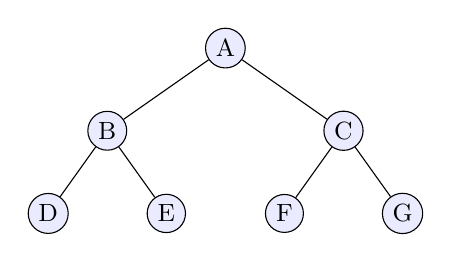
\begin{tikzpicture}[level distance=1.05cm,
  level 1/.style={sibling distance=3cm},
  level 2/.style={sibling distance=1.5cm},
  every node/.style={circle,draw,fill=blue!8,inner sep=1.8pt,font=\small}]
  \node {A}
    child {node {B}
      child {node {D}}
      child {node {E}}}
    child {node {C}
      child {node {F}}
      child {node {G}}};
\end{tikzpicture}
\end{center}

Postorder: $\mathbf{D\;E\;B\;F\;G\;C\;A}$.

\textbf{(b)} Pada pohon $m$-ari penuh, setiap simpul internal memiliki tepat $m$
anak, dan setiap simpul selain akar adalah anak dari tepat satu simpul.
Maka banyaknya simpul bukan akar $= m\,i$, sehingga
\[
n = m\,i + 1 .
\]
Karena $n = i + \ell$ (setiap simpul internal atau daun),
\[
\ell = n - i = m\,i + 1 - i = (m-1)\,i + 1 . \qquad \blacksquare
\]

\textbf{(c)} Urutkan sisi menaik:
$BC(1),\; BD(2),\; EF(2),\; AC(3),\; AB(4),\; CD(4),\; CE(5),\; DF(6),\; DE(7)$.

\begin{center}
\begin{tabular}{clcl}
\toprule
Langkah & Sisi (bobot) & Status & Keterangan\\
\midrule
1 & $BC$ (1) & diterima & komponen $\{B,C\}$\\
2 & $BD$ (2) & diterima & komponen $\{B,C,D\}$\\
3 & $EF$ (2) & diterima & komponen $\{E,F\}$\\
4 & $AC$ (3) & diterima & komponen $\{A,B,C,D\}$\\
5 & $AB$ (4) & \textbf{ditolak} & membentuk sirkuit\\
6 & $CD$ (4) & \textbf{ditolak} & membentuk sirkuit\\
7 & $CE$ (5) & diterima & seluruh simpul terhubung (5 sisi)\\
\bottomrule
\end{tabular}
\end{center}

MST $= \{BC, BD, EF, AC, CE\}$ dengan bobot total
$1 + 2 + 2 + 3 + 5 = \mathbf{13}$.

\jawab{15}
\textbf{(a)} Induksi pada $|V| = n$.

\emph{Basis} $n = 1$: $\chi(G) = 1 \le \Delta(G) + 1 = 1$.

\emph{Langkah}: andaikan berlaku untuk semua graf dengan $n$ simpul. Ambil $G$
dengan $n+1$ simpul dan pilih sembarang simpul $v$. Graf $G - v$ memiliki $n$
simpul dan $\Delta(G-v) \le \Delta(G)$, sehingga menurut hipotesis induksi
$G - v$ dapat diwarnai dengan $\Delta(G) + 1$ warna. Kembalikan $v$: simpul $v$
bertetangga dengan paling banyak $\Delta(G)$ simpul, sehingga paling banyak
$\Delta(G)$ warna terpakai di sekitarnya. Karena tersedia $\Delta(G) + 1$ warna,
selalu ada minimal satu warna yang bebas untuk $v$. $\blacksquare$

\textbf{(b)}
\begin{itemize}[leftmargin=*,nosep]
  \item $\chi(K_{3,4}) = 2$. Graf bipartit tak kosong selalu berbilangan kromatik 2
        (warnai tiap partisi dengan satu warna; tidak bisa 1 karena ada sisi).
  \item $\chi(C_7) = 3$. Siklus berpanjang ganjil tidak bipartit, jadi $\chi \ge 3$;
        pewarnaan bergantian dengan satu simpul warna ketiga menunjukkan $\chi \le 3$.
  \item $\chi(W_5) = 4$. Simpul pusat bertetangga dengan seluruh simpul $C_5$,
        sehingga warnanya harus berbeda dari semua warna siklus; karena
        $\chi(C_5) = 3$, diperoleh $\chi(W_5) = 3 + 1 = 4$.
\end{itemize}

\textbf{(c)} Bentuk graf konflik $G_c$ dengan simpul $M_1,\dots,M_7$ dan sisi
sesuai daftar konflik; slot ujian $=$ warna. Pewarnaan valid dengan 3 warna:

\begin{center}
\begin{tabular}{lccccccc}
\toprule
Mata kuliah & $M_1$ & $M_2$ & $M_3$ & $M_4$ & $M_5$ & $M_6$ & $M_7$\\
\midrule
Slot & 1 & 2 & 3 & 2 & 3 & 1 & 2\\
\bottomrule
\end{tabular}
\end{center}

Semua 12 pasangan konflik menerima slot berbeda (silakan verifikasi satu per satu),
jadi $\chi(G_c) \le 3$. Sebaliknya $M_1, M_2, M_3$ saling berkonflik dan
membentuk segitiga ($K_3$), sehingga $\chi(G_c) \ge 3$. Jadi jumlah slot minimum
adalah $\mathbf{3}$.


\vspace{1cm}
\begin{center}
\rule{0.4\textwidth}{0.4pt}\\
\textit{--- Selesai ---}
\end{center}

\end{document}